%!TEX program = xelatex
\documentclass[12pt, a4paper, openany]{book}

%!TEX program = xelatex
%% ================================================================
%%  PREAMBLE — shared formatting for the lecture-notes book
%% ================================================================

\usepackage{geometry}
\geometry{
  top    = 2.8cm,
  bottom = 2.5cm,
  left   = 3.0cm,
  right  = 2.5cm,
  headheight = 25pt,
  headsep    = 0.8cm,
  footskip   = 1.0cm
}

%% Typography
\usepackage{microtype}
\emergencystretch = 2em
\tolerance        = 800
\widowpenalty     = 10000
\clubpenalty      = 10000

%% Colours — Berkeley blue + California gold accent
\usepackage{xcolor}
\definecolor{berkeleyblue}{HTML}{003262}
\definecolor{californiagold}{HTML}{FDB515}
\definecolor{darkgold}{HTML}{C8930A}
\definecolor{lightbg}{HTML}{F7F9FC}
\definecolor{rulegray}{HTML}{BBBBBB}
\definecolor{noteblue}{HTML}{EBF4FF}
\definecolor{noteborder}{HTML}{4A90D9}
\definecolor{warningbg}{HTML}{FFF8E1}
\definecolor{warningborder}{HTML}{E6A817}
\definecolor{tipbg}{HTML}{F0FFF4}
\definecolor{tipborder}{HTML}{38A169}
\definecolor{codebg}{HTML}{F8F8F8}
\definecolor{codeframe}{HTML}{D0D0D0}
\definecolor{quotebg}{HTML}{FAF7F0}
\definecolor{quoteborder}{HTML}{B59410}
\definecolor{deflbg}{HTML}{F5F0FF}
\definecolor{deflborder}{HTML}{6B46C1}

%% Packages
\usepackage{graphicx}
\usepackage{float}
\usepackage{booktabs}
\usepackage{array}
\usepackage{titlesec}
\usepackage{mdframed}
\usepackage{enumitem}
\usepackage{fancyhdr}
\usepackage{parskip}
\usepackage{tikz}
\usepackage{amsmath}
\usepackage{amssymb}
\usepackage{listings}
\usepackage{multicol}
\usepackage{caption}
\usepackage{tabularx}
\usepackage{longtable}
\usepackage{epigraph}
\usepackage{hyperref}

\usetikzlibrary{shapes,arrows.meta,positioning,fit,backgrounds,calc}

%% Fonts (XeLaTeX)
\usepackage{fontspec}
\setmainfont{LinLibertine_R.otf}[
  Path           = fonts/,
  BoldFont       = LinLibertine_RB.otf,
  ItalicFont     = LinLibertine_RI.otf,
  BoldItalicFont = LinLibertine_RBI.otf
]
\setsansfont{LinBiolinum_R.otf}[
  Path           = fonts/,
  BoldFont       = LinBiolinum_RB.otf,
  ItalicFont     = LinBiolinum_RI.otf
]

\graphicspath{{images/}}

%% Hyperref
\hypersetup{
  colorlinks = true,
  linkcolor  = berkeleyblue,
  urlcolor   = darkgold,
  citecolor  = berkeleyblue,
  pdftitle   = {Fundamentals of Data Engineering — Lecture Notes},
  pdfauthor  = {Mahmoud Salem},
  pdfsubject = {Personal study notes on Reis & Housley (O'Reilly, 2022)}
}

%% Caption styling
\captionsetup{
  font      = {small},
  labelfont = {bf, color=berkeleyblue},
  textfont  = {it},
  format    = hang,
  margin    = 0.8cm
}

%% Section formatting
\titleformat{\chapter}[display]
  {\normalfont\Huge\bfseries\color{berkeleyblue}}
  {\filright\Large\textsc{Chapter}~\thechapter}
  {0.6em}
  {\filright}
  [\vspace{4pt}{\color{californiagold}\titlerule[2pt]}]

\titleformat{\section}
  {\Large\bfseries\color{berkeleyblue}}
  {\thesection}{0.8em}{}
  [\vspace{2pt}{\color{californiagold}\titlerule[1.5pt]}]

\titleformat{\subsection}
  {\large\bfseries\color{berkeleyblue}}
  {\thesubsection}{0.8em}{}
  [\vspace{1pt}{\color{californiagold}\titlerule[0.8pt]}]

\titleformat{\subsubsection}
  {\normalsize\bfseries\color{berkeleyblue}}
  {\thesubsubsection}{0.8em}{}

\titlespacing*{\section}      {0pt}{2.0ex plus 0.6ex minus 0.2ex}{1.0ex plus 0.3ex}
\titlespacing*{\subsection}   {0pt}{1.5ex plus 0.5ex minus 0.1ex}{0.8ex plus 0.2ex}
\titlespacing*{\subsubsection}{0pt}{1.2ex plus 0.4ex}{0.5ex plus 0.1ex}

%% Header / footer
\pagestyle{fancy}
\fancyhf{}
\fancyhead[L]{\small\color{berkeleyblue}\nouppercase{\leftmark}}
\fancyhead[R]{\small\color{californiagold}\thepage}
\fancyfoot[C]{}
\renewcommand{\headrulewidth}{0.5pt}
\renewcommand{\headrule}{%
  \hbox to\headwidth{\color{californiagold}\leaders\hrule height \headrulewidth\hfill}}
\renewcommand{\footrulewidth}{0pt}

\fancypagestyle{plain}{%
  \fancyhf{}%
  \fancyfoot[C]{\small\color{berkeleyblue}\thepage}%
  \renewcommand{\headrulewidth}{0pt}%
}

\renewcommand{\sectionmark}[1]{\markboth{#1}{}}
\renewcommand{\subsectionmark}[1]{\markboth{\thesubsection\ #1}{}}

%% Box environments
\newmdenv[
  backgroundcolor = noteblue,
  linewidth       = 2.5pt,
  linecolor       = noteborder,
  leftline=true, rightline=false, topline=false, bottomline=false,
  innertopmargin  = 10pt, innerbottommargin = 10pt,
  innerleftmargin = 14pt, innerrightmargin  = 10pt,
  skipabove = 10pt, skipbelow = 10pt
]{notebox}

\newmdenv[
  backgroundcolor = tipbg,
  linewidth       = 2.5pt,
  linecolor       = tipborder,
  leftline=true, rightline=false, topline=false, bottomline=false,
  innertopmargin  = 10pt, innerbottommargin = 10pt,
  innerleftmargin = 14pt, innerrightmargin  = 10pt,
  skipabove = 10pt, skipbelow = 10pt
]{tipbox}

\newmdenv[
  backgroundcolor = warningbg,
  linewidth       = 2.5pt,
  linecolor       = warningborder,
  leftline=true, rightline=false, topline=false, bottomline=false,
  innertopmargin  = 10pt, innerbottommargin = 10pt,
  innerleftmargin = 14pt, innerrightmargin  = 10pt,
  skipabove = 10pt, skipbelow = 10pt
]{warnbox}

\newmdenv[
  backgroundcolor = quotebg,
  linewidth       = 2.5pt,
  linecolor       = quoteborder,
  leftline=true, rightline=false, topline=false, bottomline=false,
  innertopmargin  = 10pt, innerbottommargin = 10pt,
  innerleftmargin = 16pt, innerrightmargin  = 12pt,
  skipabove = 12pt, skipbelow = 12pt
]{quotebox}

\newmdenv[
  backgroundcolor = deflbg,
  linewidth       = 2.5pt,
  linecolor       = deflborder,
  leftline=true, rightline=false, topline=false, bottomline=false,
  innertopmargin  = 10pt, innerbottommargin = 10pt,
  innerleftmargin = 14pt, innerrightmargin  = 10pt,
  skipabove = 10pt, skipbelow = 10pt
]{defbox}

%% Code listings
\lstset{
  basicstyle       = \small\ttfamily,
  backgroundcolor  = \color{codebg},
  frame            = single,
  rulecolor        = \color{codeframe},
  breaklines       = true,
  breakatwhitespace= true,
  tabsize          = 4,
  showstringspaces = false,
  numbers          = left,
  numberstyle      = \tiny\color{rulegray},
  numbersep        = 8pt,
  xleftmargin      = 16pt,
  xrightmargin     = 8pt,
  aboveskip        = 10pt,
  belowskip        = 10pt,
  framexleftmargin = 6pt,
  captionpos       = b
}

%% Convenience macros
\newcommand{\term}[1]{\textit{\textbf{#1}}}
\newcommand{\emphterm}[1]{\textbf{\color{berkeleyblue}#1}}
\newcommand{\code}[1]{\texttt{#1}}

%% Pull-quote (epigraph) styling
\setlength{\epigraphwidth}{0.78\textwidth}
\renewcommand{\epigraphflush}{flushright}
\renewcommand{\epigraphsize}{\small\itshape}
\renewcommand{\textflush}{flushepinormal}
\renewcommand{\sourceflush}{flushright}


\begin{document}

%% ─── TITLE PAGE ─────────────────────────────────────────────
\begin{titlepage}
\begin{tikzpicture}[remember picture, overlay]
  \fill[berkeleyblue]
    (current page.south west) rectangle (current page.north east);

  %% Top gold bar
  \fill[californiagold]
    ([yshift=-3.2cm]current page.north west) rectangle
    ([yshift=-3.35cm]current page.north east);

  %% Thin secondary line
  \fill[californiagold, opacity=0.5]
    ([yshift=-3.6cm]current page.north west) rectangle
    ([yshift=-3.62cm]current page.north east);

  %% Decorative giant text
  \node[anchor=west, text=white, opacity=0.08,
        font=\fontsize{180}{200}\selectfont\bfseries]
    at ([xshift=0.6cm, yshift=-10cm]current page.north west)
    {DE};

  %% Top label
  \node[anchor=west, text=californiagold!90, font=\small\sffamily]
    at ([xshift=2.5cm, yshift=-4.6cm]current page.north west)
    {LECTURE NOTES \textbullet{} VOLUME I};

  %% Main title
  \node[anchor=west, text=californiagold,
        font=\fontsize{34}{40}\selectfont\bfseries,
        text width=16cm]
    at ([xshift=2.5cm, yshift=-7.0cm]current page.north west)
    {Fundamentals of\\Data Engineering};

  %% Subtitle
  \node[anchor=west, text=white,
        font=\fontsize{17}{22}\selectfont\itshape,
        text width=16cm]
    at ([xshift=2.5cm, yshift=-10.7cm]current page.north west)
    {A study companion to the book};

  %% Description line
  \node[anchor=west, text=white!75,
        font=\normalsize, text width=16cm]
    at ([xshift=2.5cm, yshift=-11.7cm]current page.north west)
    {by Joe Reis \& Matt Housley --- O'Reilly Media, 2022};

  %% Decorative separator
  \fill[californiagold, opacity=0.35]
    ([yshift=-13.4cm, xshift=2.5cm]current page.north west) rectangle
    ([yshift=-13.43cm, xshift=-2.5cm]current page.north east);

  %% Author block
  \node[anchor=west, text=californiagold!90, font=\small\sffamily]
    at ([xshift=2.5cm, yshift=-14.4cm]current page.north west)
    {AUTHORED BY};

  \node[anchor=west, text=white,
        font=\fontsize{20}{24}\selectfont\bfseries]
    at ([xshift=2.5cm, yshift=-15.4cm]current page.north west)
    {Mahmoud~Salem};

  \node[anchor=west, text=white!75, font=\small,
        text width=16cm]
    at ([xshift=2.5cm, yshift=-16.3cm]current page.north west)
    {\href{https://www.linkedin.com/in/mahmoudalysalem}{linkedin.com/in/mahmoudalysalem}};

  %% Bottom gold bar
  \fill[californiagold]
    ([yshift=2cm]current page.south west) rectangle
    ([yshift=2.15cm]current page.south east);

  %% Thin secondary bottom line
  \fill[californiagold, opacity=0.5]
    ([yshift=1.75cm]current page.south west) rectangle
    ([yshift=1.77cm]current page.south east);

  %% Footer line
  \node[anchor=south, text=white!55, font=\small\sffamily,
        text width=18cm, align=center]
    at ([yshift=2.55cm]current page.south)
    {PREFACE \quad\textbullet\quad CHAPTER 1: DATA ENGINEERING DESCRIBED};
\end{tikzpicture}
\end{titlepage}

%% ─── COLOPHON / ABOUT THESE NOTES ───────────────────────────
\thispagestyle{empty}
\vspace*{2cm}
{\color{berkeleyblue}\Large\bfseries About these notes}\\
{\color{californiagold}\rule{6cm}{1pt}}

\vspace{1em}
\noindent These are my personal study notes for \emph{Fundamentals of Data Engineering} by Joe Reis and Matt Housley (O'Reilly Media, 2022). I'm working through the book chapter by chapter and writing down what I want to remember in my own words: the ideas that struck me, the parts that took a second pass to click, and the connections I made to things I've read elsewhere.

\vspace{1em}
\noindent The notes are not a substitute for the book. They're more like a long conversation with myself about it — what the authors said, what I think about it, and the bits of context (papers, blog posts, war stories) I went looking for to fill in the gaps. If a passage here sparks something, the next stop should be the original chapter.

\vspace{1em}
\noindent The original figures from the book are reproduced for study purposes only. All credit for the content of \emph{Fundamentals of Data Engineering} belongs to its authors and publisher.

\vspace{1em}
\noindent
\begin{tabular}{@{}ll}
\textbf{Author of these notes:} & Mahmoud Salem \\
\textbf{LinkedIn:} & \href{https://www.linkedin.com/in/mahmoudalysalem}{linkedin.com/in/mahmoudalysalem} \\
\textbf{Source book:} & Reis \& Housley, \emph{Fundamentals of Data Engineering} \\
                      & O'Reilly Media, 2022 (ISBN 978-1098108304) \\
\textbf{Volume:} & I — Preface \& Chapter 1 \\
\end{tabular}

\clearpage

%% ─── TOC ────────────────────────────────────────────────────
\setcounter{tocdepth}{2}
\pagenumbering{roman}
\tableofcontents
\clearpage
\pagenumbering{arabic}
\setcounter{page}{1}

%% ─── CONTENT ────────────────────────────────────────────────
%% ─── PREFACE NOTES ──────────────────────────────────────────
\chapter*{Preface — My reading notes}
\addcontentsline{toc}{chapter}{Preface — My reading notes}
\markboth{Preface}{}

\epigraph{The big idea of this book is the data engineering lifecycle: data generation, storage, ingestion, transformation, and serving.}{Joe Reis \& Matt Housley}

\section*{Why I picked up this book}
\addcontentsline{toc}{section}{Why I picked up this book}

I've been around data work long enough to notice a pattern: every few years, the tools change and the job titles get reshuffled, but the underlying problems stay roughly the same. Where does the data come from? How do we store it without it rotting? How do we move it somewhere useful without breaking it? And how do we serve it to the people who actually need it — analysts, scientists, ML engineers, business stakeholders — in a form they can trust?

That's the territory \emph{Fundamentals of Data Engineering} stakes out. The authors, Joe Reis and Matt Housley, both run Ternary Data and host the \emph{Joe Reis Show} (formerly \emph{The Monday Morning Data Chat}). They're not academics writing from a distance. They've been in the trenches with clients across industries, and the book has the texture of people who've debugged things at 2~a.m. and lived to tell about it.

The reason I wanted to write these notes — rather than just reading and underlining — is that the field moves fast enough that holding onto the timeless ideas matters more than the specific tools. Snowflake, Databricks, dbt, Airflow, Kafka — those are the brand names in 2026, but the \emph{shape} of the work hasn't changed since Inmon coined "data warehouse" in 1989. Reis and Housley argue this explicitly, and I want to internalize their framework so that the next time some shiny new tool shows up I can place it on the map instead of getting swept up in the marketing.

\section*{The authors' starting position}
\addcontentsline{toc}{section}{The authors' starting position}

The opening of the preface caught my attention because it's surprisingly candid. Reis and Housley call themselves "recovering data scientists." Both of them came into the data world wanting to do machine learning and analytics, got assigned to data science projects, and then ran face-first into a wall: there was no plumbing. No reliable pipelines. No clean data. No reproducible environments. They couldn't actually do data science because the foundation under the data science wasn't there.

So they shifted. They started building the infrastructure themselves, and over time realized that the foundation work was its own discipline — a hugely underappreciated one — and that there was a lot of rich, well-paid, intellectually serious work to be done in laying that foundation. That's the origin story of this book.

\begin{quotebox}
\textbf{What strikes me about this:} the authors aren't selling data engineering as the "lowly plumbing" beneath the glamorous data science work. They're saying the plumbing \emph{is} where the leverage is. If your data foundation is wrong, no amount of fancy modeling on top can save you. I've seen this myself in projects where teams kept tuning XGBoost hyperparameters when the real problem was that half their training data had a silently broken join.
\end{quotebox}

\section*{What the book is — and isn't}
\addcontentsline{toc}{section}{What the book is — and isn't}

Reis and Housley spend an explicit section telling you what the book \emph{isn't}, which I appreciate. It's not a tutorial on a specific tool. It won't teach you Spark or Airflow or BigQuery. There are good books for that, and the authors recommend treating their book as a complement to those — a kind of architectural map you read alongside the tool-specific docs.

What it \emph{is} is a framework. The big organizing idea is the \term{data engineering lifecycle}, which has five stages and six undercurrents. The five stages are linear-ish — data flows through them — and the six undercurrents thread through every stage. I'll dig into this properly in Chapter~2, but here's the skeleton, just so I have it written down somewhere I can refer back to:

\begin{defbox}
\textbf{The five lifecycle stages}
\begin{enumerate}[leftmargin=*]
  \item \textbf{Generation} — data is produced by a source system (an application database, an IoT device, a third-party API, a CSV upload).
  \item \textbf{Storage} — somewhere has to hold the data, often in multiple places along the way.
  \item \textbf{Ingestion} — moving data from a source into the systems where the engineering team has control over it.
  \item \textbf{Transformation} — reshaping the data into a form useful for downstream consumers.
  \item \textbf{Serving} — delivering the transformed data to analysts, data scientists, ML pipelines, dashboards, or reverse-ETL flows back into operational systems.
\end{enumerate}

\textbf{The six undercurrents}
\begin{itemize}[leftmargin=*]
  \item Security
  \item Data management
  \item DataOps
  \item Data architecture
  \item Orchestration
  \item Software engineering
\end{itemize}
\end{defbox}

What's powerful about this framing is its longevity. Specific technologies churn — MapReduce was the future once, then Spark replaced it, then we got Snowflake and BigQuery and the modern data stack — but the \emph{stages} the data passes through don't change. There has always been generation, there has always been storage, there has always been some kind of ingestion-transform-serve flow. Only the names and the boundaries between them shift. If I learn the stages well, I can place any new tool on the map and know what role it's playing.

\section*{The cloud-first stance}
\addcontentsline{toc}{section}{The cloud-first stance}

The authors say they take a "cloud-first" approach without apologizing for it. That's a position worth pausing on, because it's not as obvious as it sounds.

Their argument: cloud isn't just a hosting decision, it's a structural one. When infrastructure is ephemeral and elastic, the way you design data systems changes. You stop thinking about provisioning a 16-node Hadoop cluster as a six-month capital project and start thinking of compute as a knob you can turn. You lean toward managed services, because the alternative — running your own Kafka, your own Airflow, your own Postgres at scale — is more work than most teams should be doing.

I think this is broadly right, but I want to flag a counter-current the book acknowledges briefly: there's been a noticeable backlash in 2023--2024 around cloud cost. \href{https://world.hey.com/dhh/why-we-re-leaving-the-cloud-654b47e0}{37signals' "Why we're leaving the cloud"} essay made the rounds, and the FinOps Foundation has grown into a real movement. The cloud is still the default, but the assumption that it's always cheaper has been quietly retired. I'll keep this in mind as I read the rest of the book — when the authors lean on managed services, there's an implicit cost trade-off that may not always pencil out for very high-throughput steady-state workloads.

\begin{notebox}
\textbf{For my own reading:} the cloud-first vs. on-prem debate isn't really a binary. Most large data orgs are running hybrid setups — a cloud warehouse for the analytics layer, on-prem clusters for steady-state ETL or for regulated data, and SaaS for ingestion. The interesting design question isn't "cloud or not?" but "where does each component live, and why?"
\end{notebox}

\section*{Who the book is for}
\addcontentsline{toc}{section}{Who the book is for}

The authors aim the book at three groups. The primary target is technical practitioners — software engineers, data scientists, or analysts who want to move into data engineering, plus existing data engineers who are deep in one tool but want a wider perspective. The secondary target is data leadership — team leads, directors, CTOs — who need a coherent picture of the field to make hiring and technology decisions.

I fit somewhere in that mix. I read this book partly to firm up my own mental model and partly to be able to talk about the field with senior people without getting lost in tooling-specific jargon. If you're picking these notes up cold and you've never worked with data before, I'd suggest reading the book itself first — these notes assume the reader has at least bumped into terms like ETL, data warehouse, OLAP, and BI dashboard before, even if only in passing.

\section*{Prerequisites the authors assume}
\addcontentsline{toc}{section}{Prerequisites the authors assume}

The book assumes:
\begin{itemize}[leftmargin=*]
  \item Familiarity with the kinds of data systems you'd find in a corporate environment (operational databases, warehouses, BI tools — the names will be familiar even if the details aren't).
  \item Some working knowledge of \term{SQL} and \term{Python} (or another general-purpose language).
  \item Some exposure to cloud services — AWS, Azure, GCP, Snowflake, Databricks. The authors recommend setting up free-tier accounts to play with the tools as you read.
\end{itemize}

These are the bare minimum. If you don't have them, the authors' suggestion is to read the book once for the high-level ideas and then revisit it after filling in the gaps. That's actually a defensible reading strategy for any technical book — the first pass is for the shape, the second pass is for the details.

\section*{What I expect to get out of the book}
\addcontentsline{toc}{section}{What I expect to get out of the book}

The authors lay out their expectations explicitly, and I want to capture them as a benchmark to check myself against later. By the end, I should be able to:

\begin{itemize}[leftmargin=*]
  \item \textbf{Apply data engineering thinking in any data role I'm in.} Even if my title isn't "data engineer," the lifecycle framework is useful for an analyst trying to understand why their dashboards are flaky, or for a software engineer trying to design event schemas that will hold up downstream.
  \item \textbf{Cut through the marketing.} The data tooling space is genuinely overwhelming — \href{https://mattturck.com/data2024/}{Matt Turck's annual MAD landscape} chart has crossed 2,000 logos. Having a framework for evaluating tools means I can read a vendor pitch and immediately know what stage of the lifecycle it claims to address and what I should be skeptical about.
  \item \textbf{Design end-to-end architectures} that account for the full lifecycle rather than optimizing one stage at a time.
  \item \textbf{Bake security and governance into the design from the start} rather than retrofitting them after a compliance scare.
\end{itemize}

That's the contract the book is making with me. We'll see how it pans out.

\section*{How the book is structured}
\addcontentsline{toc}{section}{How the book is structured}

The book has four parts plus two appendices. I'll plot them out so I can find my way around:

\begin{itemize}[leftmargin=*]
  \item \textbf{Part I — Foundation and Building Blocks.} Chapters 1--4.
  \begin{itemize}
    \item Ch.~1: defines data engineering and the data engineer role.
    \item Ch.~2: the data engineering lifecycle in detail.
    \item Ch.~3: what makes a "good" data architecture.
    \item Ch.~4: a framework for choosing technologies. The authors are insistent that architecture and technology are different things — a distinction many teams collapse to their detriment.
  \end{itemize}
  \item \textbf{Part II — The Lifecycle in Depth.} Chapters 5--9, one chapter per lifecycle stage. The authors call this the heart of the book, and I believe them.
  \item \textbf{Part III — Security, Privacy, and the Future.} Chapters 10--11. Security and privacy used to be afterthoughts; with GDPR, CCPA, and the recent wave of data breach legislation they're now front and centre. Chapter 11 is the authors' speculation about where the field is going.
  \item \textbf{Appendix A:} serialization and compression — surprisingly load-bearing topics for a working engineer.
  \item \textbf{Appendix B:} cloud networking — the kind of thing that bites you when you don't know it.
\end{itemize}

\section*{The conventions and callouts}
\addcontentsline{toc}{section}{The conventions and callouts}

The book uses standard O'Reilly typographical conventions — italics for new terms, monospace for code, and three callout types I'll mirror in my own notes:

\begin{tipbox}
\textbf{\color{berkeleyblue}Tip}\\
A practical suggestion or rule of thumb.
\end{tipbox}

\begin{notebox}
\textbf{\color{berkeleyblue}Note}\\
A useful aside or piece of context I want to keep handy.
\end{notebox}

\begin{warnbox}
\textbf{\color{berkeleyblue}Warning}\\
Something I should avoid, or a place where mistakes are common.
\end{warnbox}

I'll use these in my own notes too, with the same colour-coding so I can scan a chapter and pick out the practical takeaways at a glance.

\section*{The acknowledgments — and what they tell us about the field}
\addcontentsline{toc}{section}{The acknowledgments and what they tell us}

Most readers skip acknowledgments. Don't, in this case. Reis and Housley thank a small army of practitioners — Bill Inmon, Zhamak Dehghani, Maxime Beauchemin, Martin Kleppmann, Andy Petrella, Chad Sanderson, Barr Moses, Benn Stancil, Jordan Tigani — and the names are themselves a reading list. These are people whose blog posts, books, and talks have shaped the modern field. A few I want to flag for my own follow-up reading:

\begin{itemize}[leftmargin=*]
  \item \textbf{Bill Inmon} — coined "data warehouse" in 1989, wrote the foundational books on data warehousing, and is still active and contrarian. His blog and books on the data warehouse versus the data lakehouse are worth the time.
  \item \textbf{Maxime Beauchemin} — wrote \href{https://www.freecodecamp.org/news/the-rise-of-the-data-engineer-91be18f1e603/}{"The Rise of the Data Engineer"} (2017), which is essentially the manifesto that named the field, and the follow-up \href{https://maximebeauchemin.medium.com/the-downfall-of-the-data-engineer-5bfb701e5d6b}{"The Downfall of the Data Engineer"}. He also created Apache Airflow at Airbnb and Apache Superset.
  \item \textbf{Zhamak Dehghani} — coined "data mesh" in a series of \href{https://martinfowler.com/articles/data-monolith-to-mesh.html}{posts on Martin Fowler's site} (2019), and wrote the O'Reilly book on data mesh.
  \item \textbf{Martin Kleppmann} — wrote \emph{Designing Data-Intensive Applications}, which is the canonical reference for the systems-engineering side of the field. If \emph{Fundamentals of Data Engineering} is the map, Kleppmann's book is the topology.
  \item \textbf{Barr Moses} — co-founded Monte Carlo and gave "data observability" its current shape.
  \item \textbf{Jordan Tigani} — built BigQuery at Google, then went on to argue that \href{https://motherduck.com/blog/big-data-is-dead/}{"Big data is dead"} (2023), which is a fascinating counterpoint to the big-data orthodoxy of the previous decade.
\end{itemize}

The authors interviewed and shaped the book around these people. Reading the book without at least sampling the underlying voices is leaving leverage on the table.

\section*{Videos and talks worth your time}
\addcontentsline{toc}{section}{Videos and talks worth your time}

Books are great, but a lot of the practitioner wisdom in this field lives in conference talks, podcasts, and YouTube. Here's a starter playlist I want to revisit while reading the book — paired with the topics they pair best with.

\begin{itemize}[leftmargin=*]
  \item \textbf{The Joe Reis Show} (formerly \emph{The Monday Morning Data Chat}). The author Joe Reis runs a long-form interview show with practitioners across the field. \href{https://www.youtube.com/@JoeReisData}{youtube.com/@JoeReisData} and on every podcast platform. If you only listen to one episode, the \emph{Bill Inmon} conversation is a master class on the historical roots of the field.
  \item \textbf{Andy Pavlo's CMU Database Group lectures.} The CMU \emph{Intro to Database Systems} (15-445) and \emph{Advanced Database Systems} (15-721) lectures are on \href{https://www.youtube.com/@CMUDatabaseGroup}{YouTube} for free. Pavlo's tour of the database world is the best free upskill in the systems side of data work, period. The 15-721 series in particular goes through OLAP, vectorisation, query optimisation, and the modern lakehouse stack.
  \item \textbf{Maxime Beauchemin --- ``The Rise of the Data Engineer''} talks. Several conference recordings exist; the Coalesce 2020 keynote is one of the better ones. Pairs with the article of the same name.
  \item \textbf{Zhamak Dehghani on Data Mesh.} Her \href{https://www.youtube.com/watch?v=TVxdW2gG3X8}{InfoQ talk on data mesh} is the cleanest one-hour summary of the architectural pattern she introduced.
  \item \textbf{Martin Kleppmann's talks.} \emph{Designing Data-Intensive Applications} the talk version: \href{https://www.youtube.com/watch?v=v2RJ1XMkPvs}{``Turning the database inside out''} (Strange Loop 2014) is the seven-year-old talk that still defines how to think about streams and materialised views.
  \item \textbf{Andrew Ng on Data-Centric AI.} A short but important shift in mindset: better data beats better models. \href{https://www.youtube.com/watch?v=06-AZXmwHjo}{``A Chat with Andrew Ng on MLOps''} is the most circulated version.
  \item \textbf{DataEng Conf, Coalesce, Subsurface, Data Council.} Four conferences worth tracking. Talks from each show up on YouTube within a few weeks of the event.
\end{itemize}

\section*{Heading into Chapter 1}
\addcontentsline{toc}{section}{Heading into Chapter 1}

The preface ends and Chapter 1 begins. Chapter 1's job is to define data engineering — the term, the role, the relationship with adjacent roles, and the historical arc that produced the field as it exists today. I'll pick that up next.

\clearpage

%% ─── CHAPTER 1 NOTES ────────────────────────────────────────
\chapter{Data Engineering Described}
\markboth{Chapter 1 — Data Engineering Described}{}

\epigraph{Data engineering is one of the hottest fields in data and technology, and for a good reason. It builds the foundation for data science and analytics in production.}{Joe Reis \& Matt Housley}

\section*{Opening — what this chapter is doing}
\addcontentsline{toc}{section}{Opening — what this chapter is doing}

The first chapter of any technical book has a thankless job: define the field, sketch its boundaries, locate it on a wider map, and do all of that without boring readers who already work in it or losing readers who don't. Reis and Housley take a swing at this by answering four interlocking questions:

\begin{enumerate}[leftmargin=*]
  \item \textbf{What is data engineering?} A definition that's broad enough to survive tooling churn and narrow enough to actually mean something.
  \item \textbf{How did we get here?} A short history of the field — data warehousing in the 1980s, the dot-com aftermath, big data, the cloud, and the present moment.
  \item \textbf{What does a data engineer actually do?} The skill set, the responsibilities, and the difference between two archetypes the authors call type A and type B.
  \item \textbf{Who do data engineers work with?} The web of upstream and downstream stakeholders, including the tangled question of where data engineering ends and data science, ML engineering, software engineering, or analytics begins.
\end{enumerate}

I'll work through each in turn and add my own notes — definitions, mental models, references to related reading, and the bits where I think the authors gloss over something that deserves a closer look.

\section{What is data engineering?}

\subsection{The definitional mess}

A confession from the authors I appreciated: even in early 2022, a Google search for \emph{"what is data engineering?"} returned over 91{,}000 unique results. There's no standardised definition. Different practitioners describe the role through different lenses, and they're often all partially right.

The book quotes four definitions from working practitioners, and reading them back-to-back is a useful exercise because each one tells you something about what mattered to the person writing it:

\begin{quotebox}
\textbf{AlexSoft} — "Data engineering is a set of operations aimed at creating interfaces and mechanisms for the flow and access of information. \dots Data engineers set up and operate the organization's data infrastructure, preparing it for further analysis."
\end{quotebox}

This one focuses on \emph{infrastructure}. Data engineering is plumbing — building and maintaining the systems through which data flows. It's accurate as far as it goes, but it makes the role sound like ops work, which undersells the design and modelling components.

\begin{quotebox}
\textbf{Jesse Anderson} — splits data engineering into "SQL-focused" (relational databases, ETL, BI) and "Big Data–focused" (Hadoop, Spark, Flink, distributed processing).
\end{quotebox}

Anderson's split was useful in 2018, less so now. The two worlds Reis and Housley describe have largely merged — modern warehouses like Snowflake and BigQuery handle petabytes with SQL, while big-data frameworks like Spark have first-class SQL APIs. The dichotomy describes the field of seven years ago, not the field of today. But it's a good reminder of \emph{how recent} the field is.

\begin{quotebox}
\textbf{Maxime Beauchemin} — "Data engineering \dots could be thought of as a superset of business intelligence and data warehousing that brings more elements from software engineering. This discipline also integrates specialization around the operation of so-called 'big data' distributed systems."
\end{quotebox}

Beauchemin's lens is the historical one. He's saying: take BI and warehousing, layer on the discipline of software engineering, then add the distributed-systems toolkit. He'd know — he wrote the manifesto piece "The Rise of the Data Engineer" in 2017 and built Airflow at Airbnb. (See his article at \href{https://www.freecodecamp.org/news/the-rise-of-the-data-engineer-91be18f1e603/}{freecodecamp.org/the-rise-of-the-data-engineer}.)

\begin{quotebox}
\textbf{Lewis Gavin} — "Data engineering is all about the movement, manipulation, and management of data."
\end{quotebox}

The shortest of the four. \emph{Movement} (ingestion, transport), \emph{manipulation} (transformation), \emph{management} (governance, quality, lifecycle). It's a useful mnemonic, even if it leaves out the design work.

\subsection{The book's definition}

After looking at all four, Reis and Housley land on their own working definition, and this is the one I want to commit to memory because the rest of the book depends on it:

\begin{defbox}
\textbf{Data engineering} is the development, implementation, and maintenance of \emph{systems and processes} that take in \emph{raw data} and produce \emph{high-quality, consistent information} that supports \emph{downstream use cases} such as analysis and machine learning. Data engineering is the \emph{intersection} of security, data management, DataOps, data architecture, orchestration, and software engineering.

A \textbf{data engineer} manages the data engineering lifecycle, beginning with getting data from source systems and ending with serving data for use cases such as analysis or machine learning.
\end{defbox}

A few things in this definition that I want to note explicitly:

\begin{itemize}[leftmargin=*]
  \item \textbf{"Systems and processes."} It's not just code. It's not just infrastructure. It's both, plus the human and organisational processes around them. A data engineer who can write a great pipeline but can't get stakeholders to agree on what "active user" means is going to fail.
  \item \textbf{"Raw data" $\to$ "high-quality, consistent information."} This is the value-creation framing. Data engineering takes a low-trust input and produces a high-trust output. The work is the difference.
  \item \textbf{"Downstream use cases."} The point of data engineering is not to engineer data for its own sake. The data only matters because someone or something — an analyst, a model, a business process, a customer-facing feature — is going to use it.
  \item \textbf{"Intersection."} The authors are explicit that data engineering is not a single discipline but a junction of six others. That's why the role is hard to pin down: you're expected to be conversant in security, data management, DataOps, architecture, orchestration, and software engineering, even though no single person can be deeply expert in all six.
\end{itemize}

\subsection{The data engineering lifecycle}

\begin{figure}[H]
  \centering
  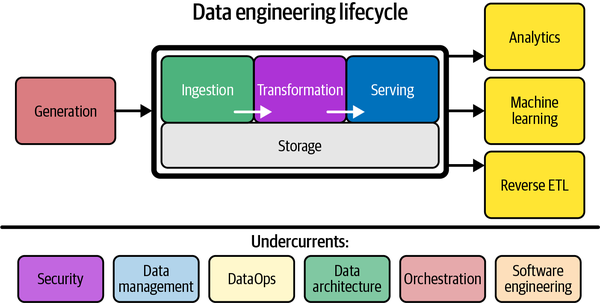
\includegraphics[width=0.92\textwidth, keepaspectratio]{fig_01_01_data_engineering_lifecycle.png}
  \caption{The data engineering lifecycle. Five stages from generation to serving, with six undercurrents threading through every stage. Reproduced from Reis \& Housley (2022), Figure~1-1.}
  \label{fig:lifecycle}
\end{figure}

Figure~\ref{fig:lifecycle} is the diagram I'll come back to most often in this book, so I want to make sure I read it carefully. The horizontal dimension shows the five \emph{stages} that data passes through:

\begin{enumerate}[leftmargin=*]
  \item \textbf{Generation.} A source system produces data. This could be an OLTP database behind a web app, an event stream from a mobile client, an IoT sensor, a third-party SaaS API, or a flat file uploaded by a vendor.
  \item \textbf{Storage.} Data has to live somewhere — and usually in several places along the way. The book treats storage as a stage but also as something that wraps around all the other stages, which is why the diagram visualises it as the underlying base.
  \item \textbf{Ingestion.} Moving data from a source system into a system the data team controls. This is where things break most often, in my experience: schemas drift, sources go down, formats change without warning.
  \item \textbf{Transformation.} Reshaping data into something useful — joining, deduplicating, applying business logic, building aggregations, conforming to a data model.
  \item \textbf{Serving.} Delivering the transformed data to its consumers — BI dashboards, ML training pipelines, reverse-ETL flows back into operational systems, or API endpoints that downstream applications call.
\end{enumerate}

The vertical dimension — the \emph{undercurrents} — is what I find most interesting about the model, because it's how the authors avoid the trap of treating data engineering as a strictly linear pipeline-building activity. There are six undercurrents:

\begin{itemize}[leftmargin=*]
  \item \textbf{Security} — encryption, access control, secrets management, compliance with PII rules.
  \item \textbf{Data management} — quality, governance, lineage, cataloging, master data management.
  \item \textbf{DataOps} — the cultural and practice layer that brings DevOps thinking (CI/CD, observability, on-call) to data systems.
  \item \textbf{Data architecture} — the higher-level design of how systems fit together.
  \item \textbf{Orchestration} — coordinating tasks and dependencies across systems (Airflow, Dagster, Prefect, Argo, Step Functions).
  \item \textbf{Software engineering} — version control, testing, code review, modular design. The book is emphatic that data engineers are software engineers, not just SQL writers.
\end{itemize}

Every undercurrent applies at every stage. Security in ingestion is different from security in serving, but neither can be skipped. DataOps in transformation is different from DataOps in storage, but both matter. The framework is genuinely useful as a checklist when you're designing or reviewing an architecture: for each stage, run through the six undercurrents and ask whether you've thought about each one.

\begin{notebox}
\textbf{Where this comes from.} The "lifecycle plus undercurrents" model isn't unique to this book — it borrows from a long tradition of process frameworks in software engineering (think SDLC) and data management (think DAMA-DMBOK). What's new is the specific framing for data engineering and the way it accommodates both the modern data stack and older on-prem patterns. We get the full treatment in Chapter~2.
\end{notebox}

\subsection{Evolution of the data engineer}

A bit of history. The authors warn that this isn't a history lesson, but they want us to understand where the field came from because, as they put it, "what's old is new again." There are roughly four eras to walk through.

\subsubsection{The early days — 1980 to 2000}

The data engineer's lineage starts with \term{data warehousing}. The relational database and SQL were developed at IBM in the 1970s, popularised by Oracle, and by the late 1980s businesses had enough operational data to want a separate system optimised for analysis. Bill Inmon coined the term "data warehouse" in 1989, and around the same time Ralph Kimball developed the dimensional modelling approach (star schemas, fact tables, dimension tables) that's still in active use forty years later.

Two competing modelling philosophies emerged from this period and are worth knowing the difference between:

\begin{itemize}[leftmargin=*]
  \item \textbf{Inmon} — top-down. Build a single, normalised, enterprise-wide data warehouse first, then derive subject-specific data marts from it. Think of it as a corporate single source of truth.
  \item \textbf{Kimball} — bottom-up. Build dimensional data marts directly, using a "bus architecture" of conformed dimensions to integrate them. Faster to deliver value, but requires careful coordination to avoid drift.
\end{itemize}

If you ever find yourself in an argument about whether "the warehouse" should be normalised (3NF) or dimensional (star schema), this is the argument you've stumbled into. Both approaches work. The right answer depends on the organisation.

The 1990s also brought \term{massively parallel processing} (MPP) databases — Teradata, Netezza, Greenplum — which used multiple processors to handle volumes that single-server databases choked on. These are the direct ancestors of today's cloud data warehouses (Snowflake, BigQuery, Redshift), even though the marketing has moved on.

Then the internet went mainstream around 1995, and a generation of web-first companies — AOL, Yahoo, Amazon — started generating data at scales the existing technology had never anticipated. That set up the next era.

\subsubsection{The early 2000s — birth of contemporary data engineering}

The dot-com bust left a small cluster of survivors (Yahoo, Google, Amazon) that grew into the platform companies we know today. They were generating staggering amounts of data and were running into hard scaling walls with traditional relational databases. They needed something new.

Two papers from Google changed the field:

\begin{itemize}[leftmargin=*]
  \item \textbf{The Google File System} (2003). A distributed file system designed for cheap commodity hardware, with redundancy built in.
  \item \textbf{MapReduce: Simplified Data Processing on Large Clusters} (2004). A programming model for processing huge data sets in parallel across clusters of inexpensive machines.
\end{itemize}

These papers are still worth reading. They're \href{https://research.google/pubs/the-google-file-system/}{available on Google's research site}, and they're not particularly long. They're also the cultural origin of the field: when engineers at Yahoo read them, they built an open-source implementation called \textbf{Apache Hadoop} (initial release 2006), which became the standard distributed-data platform for the next decade.

Around the same time, Amazon launched \textbf{Amazon Web Services} (AWS) — first S3 in 2006, then EC2, then DynamoDB, and on. The pitch was simple: stop buying hardware, rent compute and storage by the hour. AWS effectively invented the public cloud as a commercial offering, and Microsoft and Google followed with Azure and GCP.

You can draw a straight line from these two innovations — Hadoop and AWS — to almost everything that came after. The big-data era and the cloud era both started here, and they fused: the cloud became the default place to run big data workloads, and the modern data stack runs almost entirely on cloud infrastructure.

\subsubsection{The 2000s and 2010s — big data engineering}

\begin{figure}[H]
  \centering
  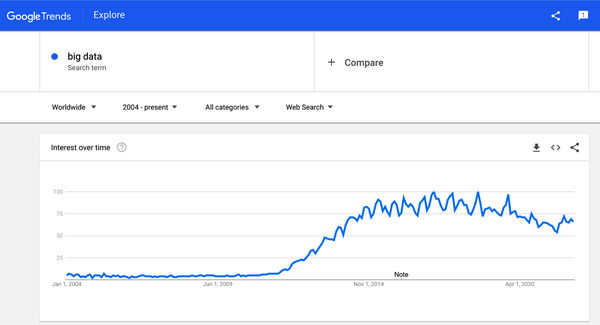
\includegraphics[width=0.85\textwidth, keepaspectratio]{fig_01_02_big_data_search_trend.png}
  \caption{Google search interest for the term "big data" over time. The arc is a perfect bubble: rapid rise from 2010, peak around 2015, slow decline as the term lost meaning. Reproduced from Reis \& Housley (2022), Figure~1-2.}
  \label{fig:bigdata-trend}
\end{figure}

Hadoop and AWS made it possible for any company — not just Google — to handle volumes that would have been impossible a decade earlier. The "big data" era was on. Engineers had a growing menu of open-source tools to work with: Apache Pig (data flow language for Hadoop), Apache Hive (SQL on Hadoop), Apache HBase (distributed key-value store), Apache Storm (stream processing), Apache Cassandra (wide-column store), Apache Spark (in-memory distributed processing), Presto (interactive SQL), and many more.

The role of "big data engineer" appeared. The job was to operate massive clusters, write MapReduce/Spark jobs, and deliver data at scale. It required a strange mix of skills: software engineering, distributed systems, low-level cluster admin, and a tolerance for tools that could be brittle and complicated.

But "big data" became a victim of its own marketing. The authors quote a line from Dan Ariely that captured the moment perfectly: \emph{"Big data is like teenage sex: everyone talks about it, nobody really knows how to do it, everyone thinks everyone else is doing it, so everyone claims they are doing it."} Companies were spinning up Hadoop clusters to process gigabytes of data. The hype far outpaced reality.

What killed the term — at least as a useful one — was \textbf{simplification}. Cloud-native services (BigQuery, Snowflake, EMR, Dataflow) abstracted away most of the operational pain. You no longer needed a team of cluster administrators to query a petabyte; you submitted a SQL query and the cloud did the rest. By the late 2010s the term "big data" had drained of meaning. Today the authors put it bluntly: "Big data engineers are now simply data engineers."

\begin{notebox}
\textbf{Reading recommendation.} Jordan Tigani's 2023 essay \href{https://motherduck.com/blog/big-data-is-dead/}{"Big data is dead"} on the MotherDuck blog is a direct, cogent argument that for most companies the data is just not that big. He pulls real-world numbers from BigQuery and shows that 90\% of customer queries process under 100~MB. It's a great companion read to this section because it puts a precise edge on the trend Reis and Housley describe.
\end{notebox}

\subsubsection{The 2020s — engineering for the data lifecycle}

\begin{figure}[H]
  \centering
  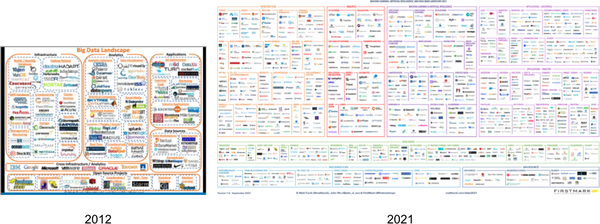
\includegraphics[width=0.92\textwidth, keepaspectratio]{fig_01_03_modern_data_tools_landscape.png}
  \caption{The modern data tooling landscape. The chart that launched a thousand vendor pitches. Reproduced from Reis \& Housley (2022), Figure~1-3.}
  \label{fig:tools-landscape}
\end{figure}

The current era is what the authors call "engineering for the data lifecycle." The shift is away from hand-managing low-level frameworks (Hadoop, Spark, Informatica) and toward composing modular, managed, abstracted services into pipelines. This is the era of:

\begin{itemize}[leftmargin=*]
  \item \textbf{The modern data stack}: a loosely-coupled set of best-of-breed tools — typically Fivetran/Airbyte for ingestion, Snowflake/BigQuery/Redshift/Databricks for storage and compute, dbt for transformation, Looker/Mode/Hex/Tableau for serving, and Airflow/Dagster/Prefect for orchestration.
  \item \textbf{ELT over ETL}: load raw data into the warehouse first, transform it inside the warehouse with SQL.
  \item \textbf{Data observability}: tools like Monte Carlo and Bigeye that monitor data quality the way Datadog monitors application health.
  \item \textbf{Data contracts and data products}: treating downstream-facing datasets as first-class APIs with explicit schemas, SLAs, and ownership.
  \item \textbf{Lakehouse architectures}: Delta Lake, Apache Iceberg, Apache Hudi — open table formats that bring warehouse-like guarantees (ACID transactions, schema evolution, time travel) to object storage.
\end{itemize}

The figure is overwhelming on purpose. Looking at it is a useful exercise — not because you should learn every logo, but because you need to feel the scale of the proliferation. The authors cite Matt Turck's annual "MAD Landscape" (Machine Learning, AI, and Data); the latest editions have well over 2{,}000 logos. Your job as a data engineer is not to know all of them. Your job is to know the categories, the trade-offs between them, and how to recognise an underwhelming tool when a vendor pitches it as essential.

The authors describe today's data engineer as a \term{data lifecycle engineer} — someone less focused on the gritty internals of any one framework and more on stitching together a coherent end-to-end flow that's secure, governed, and reliable. The role has moved up the value chain. That's a real shift, and it's why the book is structured around the lifecycle and the undercurrents rather than around any specific tool.

\subsection{Data engineering and data science}

\begin{figure}[H]
  \centering
  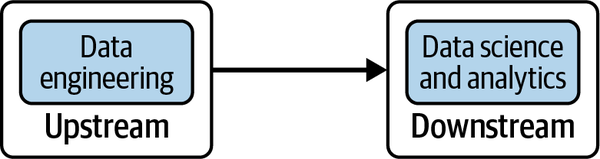
\includegraphics[width=0.85\textwidth, keepaspectratio]{fig_01_04_engineering_upstream_of_science.png}
  \caption{Data engineering sits upstream of data science. Engineers provide the inputs that scientists transform into models and analysis. Reproduced from Reis \& Housley (2022), Figure~1-4.}
  \label{fig:upstream}
\end{figure}

There's a perennial argument in tech about whether data engineering is a subset of data science or a separate discipline. Reis and Housley take a clear position: \emph{separate}. Adjacent, complementary, but separate. Data engineers sit \emph{upstream} of data scientists, providing the inputs the scientists turn into models and insights.

The diagram on data science's hierarchy of needs (Figure~\ref{fig:hierarchy}) is the killer argument for why these are distinct roles.

\begin{figure}[H]
  \centering
  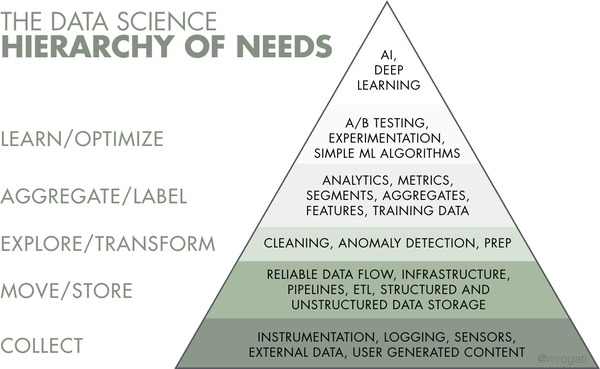
\includegraphics[width=0.78\textwidth, keepaspectratio]{fig_01_05_data_science_hierarchy_of_needs.png}
  \caption{Monica Rogati's data science hierarchy of needs (2017). AI/ML sits at the top; collection, infrastructure, and movement form the foundation. Reproduced from Reis \& Housley (2022), Figure~1-5.}
  \label{fig:hierarchy}
\end{figure}

Monica Rogati published this in 2017 in an essay titled \href{https://hackernoon.com/the-ai-hierarchy-of-needs-18f111fcc007}{"The AI Hierarchy of Needs"}. The pyramid is built like Maslow's: the lower layers have to be solid before the upper ones can do real work. From bottom to top:

\begin{enumerate}[leftmargin=*]
  \item \textbf{Collect} — instrumentation, sensors, logs, getting data from external sources.
  \item \textbf{Move/store} — reliable data flow, infrastructure, pipelines, ETL/ELT, data preparation.
  \item \textbf{Explore/transform} — cleaning, anomaly detection, prep for analysis.
  \item \textbf{Aggregate/label} — analytics, metrics, segments, training data.
  \item \textbf{Learn/optimise} — A/B testing, experimentation, simple ML.
  \item \textbf{AI/deep learning} — at the very top.
\end{enumerate}

Rogati's punchline is that companies routinely try to skip from layer 1 to layer 6, hire a deep-learning team, and then wonder why the models don't work in production. The answer is almost always that the foundation isn't there. \emph{Data scientists spend an estimated 70--80\% of their time on the bottom three layers}, doing work that would be better done by data engineers.

There's a healthy debate about whether the 80\% number is real or folklore. The book cites Leigh Dodds's 2020 piece \href{https://blog.ldodds.com/2020/01/31/do-data-scientists-spend-80-of-their-time-cleaning-data-turns-out-no/}{"Do data scientists spend 80\% of their time cleaning data? Turns out, no?"} as a contrarian view, and an Anaconda survey from 2020 put the number around 45\%. Wherever the precise figure lands, the qualitative point holds: a lot of data scientists spend a lot of time doing what is fundamentally data engineering work, and that's a misallocation.

\begin{figure}[H]
  \centering
  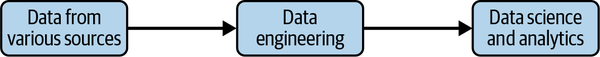
\includegraphics[width=0.92\textwidth, keepaspectratio]{fig_01_06_engineering_to_value.png}
  \caption{Data engineering bridges raw data and the value extracted from it. Reproduced from Reis \& Housley (2022), Figure~1-6.}
  \label{fig:value}
\end{figure}

The authors put it this way: data engineering "straddles the divide between getting data and getting value from data." That's a phrase worth holding onto. The moment the engineering work goes well, the science work gets dramatically more productive — because the scientists can spend their time doing science.

\section{Data engineering skills and activities}

\begin{figure}[H]
  \centering
  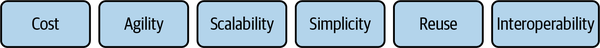
\includegraphics[width=0.92\textwidth, keepaspectratio]{fig_01_07_optimization_axes.png}
  \caption{The axes a data engineer is constantly optimising along: cost, agility, scalability, simplicity, reuse, and interoperability. Reproduced from Reis \& Housley (2022), Figure~1-7.}
  \label{fig:axes}
\end{figure}

What does a data engineer actually \emph{do}? The book frames it as constant trade-off management along six axes:

\begin{itemize}[leftmargin=*]
  \item \textbf{Cost} — total cost of ownership, opportunity cost, time-to-value.
  \item \textbf{Agility} — how quickly the system can adapt when requirements change.
  \item \textbf{Scalability} — how it behaves when data volume, velocity, or variety grows.
  \item \textbf{Simplicity} — how easy it is for someone else to operate, debug, and extend.
  \item \textbf{Reuse} — whether components can be shared across pipelines, teams, or use cases.
  \item \textbf{Interoperability} — whether the pieces play well with the rest of the ecosystem.
\end{itemize}

You can't maximise all six simultaneously. Optimising for one usually costs another. A perfectly simple pipeline is rarely the most reusable; the cheapest tool may not scale; the most scalable may be a nightmare to operate. A senior data engineer's judgement is largely a judgement about which axis to bias toward in any given situation.

The authors are clear about what's \emph{not} on this list, and it's worth flagging:

\begin{itemize}[leftmargin=*]
  \item Data engineers \textbf{don't typically build ML models}.
  \item They \textbf{don't typically build dashboards or run analyses}.
  \item They \textbf{don't typically own KPIs or business metrics}.
  \item They \textbf{don't typically write end-user-facing applications}.
\end{itemize}

A data engineer should \emph{understand} all of these — enough to talk to the people who do them — but the engineer's primary job is to deliver clean, governed, reliable data so that those other roles can do their work.

\subsection{Data maturity and the data engineer}

\begin{figure}[H]
  \centering
  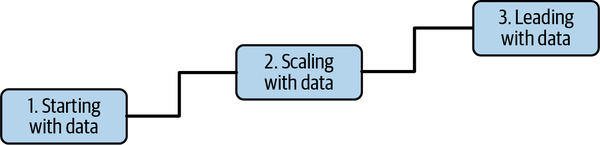
\includegraphics[width=0.92\textwidth, keepaspectratio]{fig_01_08_data_maturity_model.png}
  \caption{The book's three-stage data maturity model: starting with data, scaling with data, leading with data. Reproduced from Reis \& Housley (2022), Figure~1-8.}
  \label{fig:maturity}
\end{figure}

The work changes dramatically depending on the data maturity of the company you're in. The authors propose a simplified three-stage model — partly because more elaborate models like the CMMI Data Management Maturity (DMM) framework have too many levels to be useful for day-to-day decisions.

Critically, data maturity is \emph{not} a function of company age or revenue. A two-year-old startup running well-instrumented event pipelines and dbt models on Snowflake can have higher data maturity than a 100-year-old conglomerate still running batch ETL into an on-prem Teradata warehouse. What matters is how seriously the company takes data as a competitive weapon.

\subsubsection{Stage 1 — starting with data}

The company is in its data infancy. Goals are vague or absent. The data team is small (often a single person wearing every hat). Architecture is improvised. Most data requests are ad hoc.

A data engineer at this stage is a \emph{generalist}. The goal is to get traction quickly — produce visible wins, build trust, and lay a foundation for the next stage. The four practical priorities the book lists are worth quoting close to verbatim:

\begin{itemize}[leftmargin=*]
  \item \textbf{Get buy-in from key stakeholders} — ideally an executive sponsor for the data initiative.
  \item \textbf{Define the data architecture} — usually solo, since there's no architect on staff. Tie it to specific business goals.
  \item \textbf{Identify the data} that supports those goals.
  \item \textbf{Build a foundation} for future analysts and data scientists, even if you have to play those roles yourself in the meantime.
\end{itemize}

And the warnings:

\begin{warnbox}
\textbf{Stage 1 traps to avoid}\\
$\bullet$ \textbf{Working in a silo.} The data team that doesn't talk to the rest of the business spends months delivering things nobody wanted.\\
$\bullet$ \textbf{Jumping straight to ML.} Without a foundation, ML models will fail in production. The authors call themselves "recovering data scientists" because they've lived this.\\
$\bullet$ \textbf{Undifferentiated heavy lifting.} Don't write a custom orchestrator when Airflow exists. Don't roll your own warehouse when Snowflake exists. Custom-build only where it creates competitive advantage.\\
$\bullet$ \textbf{Quick wins without a debt-payback plan.} Quick wins almost always create technical debt. That's fine, as long as you have a plan to pay it down before it suffocates you.
\end{warnbox}

\subsubsection{Stage 2 — scaling with data}

The company has formal data practices and a real data team. The challenge is to design architectures that scale and build the cultural muscle of a data-driven organisation. Roles specialise: rather than one person doing ingestion, transformation, and serving, you have specialists in each.

A data engineer's goals at stage 2:
\begin{itemize}[leftmargin=*]
  \item Establish formal data practices (testing, code review, runbooks, on-call).
  \item Create scalable, robust architectures that won't have to be rebuilt in two years.
  \item Adopt DevOps and DataOps practices — CI/CD for data, observability, alerting.
  \item Build the systems that ML will need (feature stores, training pipelines, model serving — coordinated with the ML team where one exists).
  \item Continue to avoid undifferentiated heavy lifting.
\end{itemize}

\begin{warnbox}
\textbf{Stage 2 traps}\\
$\bullet$ \textbf{Bleeding-edge tooling for its own sake.} The dopamine rush of adopting whatever tool the FAANGs are using is real. Resist it. Most tools that big tech companies open-source were built for problems your company doesn't have.\\
$\bullet$ \textbf{The bottleneck is the team, not the cluster.} You can buy more compute. You can't easily buy more data engineers. Pick tools that don't require your team to grow linearly with data volume.\\
$\bullet$ \textbf{The "data genius" trap.} Stage 2 is where data engineers are tempted to position themselves as wizards. The authors push back hard: shift to pragmatic leadership, communicate, teach the rest of the org how to consume data.
\end{warnbox}

\subsubsection{Stage 3 — leading with data}

The company is genuinely data-driven. Pipelines are largely automated. Self-service analytics is real. Introducing a new data source takes hours, not weeks. Specialised roles continue to specialise.

The data engineer's job at this stage:
\begin{itemize}[leftmargin=*]
  \item Build automation for seamlessly onboarding new data sources.
  \item Build custom tools where they're a competitive advantage.
  \item Focus on the "enterprise-y" things — governance, lineage, master data, metadata, catalogs.
  \item Roll out tools that expose data across the organisation: catalogs (DataHub, Atlan, Amundsen), lineage tools (OpenLineage, Marquez), metadata systems.
  \item Collaborate efficiently across roles — software engineers, ML engineers, analysts.
  \item Build a culture where people across roles can talk to each other openly.
\end{itemize}

\begin{warnbox}
\textbf{Stage 3 traps}\\
$\bullet$ \textbf{Complacency.} Stage 3 isn't a fixed state. Without continuous improvement you slip back. There's a long list of formerly-stage-3 companies that woke up to find their data platform had quietly become the legacy system everyone wants to migrate off.\\
$\bullet$ \textbf{Hobby projects.} The most dangerous engineering manager is a stage-3 data eng manager with budget. The temptation to build interesting infrastructure that doesn't move the business is real. Custom-build only where it provides competitive advantage; otherwise buy or use open-source.
\end{warnbox}

\subsection{The background and skills of a data engineer}

The book is honest about the fact that data engineering doesn't have a standard curriculum. There's no "BSc in Data Engineering" the way there's a CS degree. Most working data engineers came from somewhere adjacent — software engineering, ETL development, DBA work, data analysis, data science — and self-studied their way into the field.

That self-study burden is one of the structural facts about the role. Expect to spend a lot of time reading, watching talks, doing tutorials, and building side projects. The book itself is part of that self-study, and the authors are explicit that it's a starting point rather than a complete map.

The minimum body of knowledge they think a data engineer needs:

\begin{itemize}[leftmargin=*]
  \item \textbf{Data} — best practices around data management, modelling, quality, governance.
  \item \textbf{Technology} — fluency in the major tool categories, the trade-offs between options, and the ability to evaluate new tools quickly.
  \item \textbf{Software engineering} — version control, testing, CI/CD, modular design.
  \item \textbf{DataOps} — observability, alerting, on-call, change management.
  \item \textbf{Data architecture} — system design across the lifecycle.
  \item \textbf{The consumers' perspective} — what analysts and data scientists need, and what business stakeholders care about.
\end{itemize}

The framing the authors give that I find most useful: \emph{a data engineer should view their work through both business and technical lenses simultaneously}. The best engineers I've worked with do this naturally. They can write a Spark job at 11~a.m. and present a roadmap to a CTO at 2~p.m. without losing the thread.

\subsection{Business responsibilities}

The book lists a set of "business responsibilities" that aren't unique to data engineering but matter a lot for senior people in the role:

\begin{itemize}[leftmargin=*]
  \item \textbf{Communication.} Build trust across the organisation. Pay attention to org charts, reporting lines, and where the silos are.
  \item \textbf{Scoping and gathering requirements.} Know what to build and make sure stakeholders agree.
  \item \textbf{Cultural change.} Agile, DevOps, and DataOps are cultural before they're technical. Tools alone don't fix process problems.
  \item \textbf{Cost discipline.} Time-to-value, total cost of ownership, opportunity cost. Watch the cloud bill.
  \item \textbf{Continuous learning.} Filter the new from the merely shiny. Learn how to learn.
  \item \textbf{Big-picture thinking.} The career-limiting move for a senior data engineer is to be the world's best Spark hacker who can't articulate why a business should care about Spark.
\end{itemize}

\subsection{Technical responsibilities}

The authors then turn to the technical side. The lifecycle and undercurrents are the structuring frame, but they call out specific skills worth having.

\subsubsection{Programming languages}

A perennial question: \emph{should a data engineer know how to code?} The book's answer is unambiguous: \emph{yes}. Production-grade software engineering chops are non-negotiable. The reason is simple — even with managed services and SaaS abstractions everywhere, you still write code (pipelines as code, transformations in dbt, custom orchestration logic), and you'll need to read other people's code constantly.

The authors split languages into primary and secondary tiers.

\textbf{Primary languages:}

\begin{itemize}[leftmargin=*]
  \item \textbf{SQL.} The lingua franca of the field. After being briefly sidelined in the early big-data era (when MapReduce was supposed to replace it), SQL has come roaring back. Every modern data warehouse and many streaming systems (Flink, KsqlDB) speak it. Modern dialects handle JSON, semi-structured data, window functions, recursive CTEs — there's a lot of expressive power in SQL today, and it's worth getting deep.
  \item \textbf{Python.} The "second-best language at everything." It's the glue between everything else. pandas, NumPy, Airflow, dbt-core's Jinja templating, PySpark, scikit-learn, TensorFlow, PyTorch — all Python. If you know one general-purpose language well enough to write production code, this is the one.
  \item \textbf{A JVM language (Java or Scala).} Spark, Flink, Beam, Hive, Druid, Kafka — all written on the JVM. The Python APIs work, but for performance-critical work or low-level access you'll occasionally need to drop into Scala or Java. Knowing the JVM is also worth it for reading the source of these tools when something breaks.
  \item \textbf{Bash (or PowerShell on Windows).} The Linux command line is where pipelines run. Knowing your way around \code{awk}, \code{sed}, \code{jq}, \code{find}, and the standard pipe vocabulary is a massive productivity multiplier.
\end{itemize}

\begin{tipbox}
\textbf{The unreasonable effectiveness of SQL.} The authors include a sidebar with this title — a riff on \href{https://www.youtube.com/watch?v=PlGw1HBl5p8}{Eugene Wigner's "Unreasonable Effectiveness of Mathematics in the Natural Sciences"}. SQL is a powerful, declarative, set-theoretic language that can solve a startling range of problems with very little code. The trade-off: a competent data engineer also recognises when SQL is the wrong tool — say, for an NLP pipeline that needs tokenisation and stemming — and reaches for Python or Scala instead.
\end{tipbox}

\textbf{Secondary languages} the authors mention: R, JavaScript, Go, Rust, C/C++, C\#, Julia. Which one matters depends on the company. JavaScript is common for user-defined functions in cloud warehouses. C\# and PowerShell matter heavily in Azure-heavy Microsoft shops. Go and Rust are increasingly common in newer data infrastructure projects (Materialize, InfluxDB IOx).

\subsubsection{Keeping pace}

The book has a short section on staying current that I want to keep close. The advice:

\begin{enumerate}[leftmargin=*]
  \item \textbf{Focus on fundamentals} to understand what won't change. The data engineering lifecycle, the undercurrents, the principles of system design — these have been useful for forty years and will be useful for forty more.
  \item \textbf{Pay attention to ongoing developments} to know where the field is going. Read the blogs (dbt, Snowflake, Databricks, Fivetran, the practitioner blogs at Airbnb/Uber/Netflix/Spotify). Listen to the podcasts. Attend conferences.
  \item \textbf{Filter ruthlessly.} Most new tools are noise. A few are signal. Knowing the difference is a skill.
\end{enumerate}

The Stewart Brand quote the authors include is worth remembering: \emph{"Once a new technology rolls over you, if you're not part of the steamroller, you're part of the road."} The point isn't to chase every new tool — it's to know enough to not be caught flat-footed when a real shift happens. Hadoop arrived. Spark arrived. The cloud arrived. Snowflake arrived. dbt arrived. Each of these reshaped the field. The next one is coming, and the only way to be ready for it is to stay engaged.

\subsection{The continuum of roles, type A to type B}

Job descriptions for data engineers tend to ask for everything: SQL, Python, Spark, Airflow, dbt, Snowflake, BigQuery, Kafka, Kubernetes, Terraform, ML, statistics, business acumen, communication skills, and an MBA on the side. The reality is that real data engineers tend to specialise. The book introduces a useful taxonomy borrowed from the data science world.

\begin{defbox}
\textbf{Type A — Abstraction.}\\
Avoids undifferentiated heavy lifting. Keeps architecture as simple and abstract as possible. Uses off-the-shelf products, managed services, and existing open-source tools. Doesn't reinvent wheels. Common in companies of every size and at every maturity stage. Most data engineers are type A.

\textbf{Type B — Build.}\\
Builds new tools and systems where the company's competitive advantage requires it. More common at stage 2 and stage 3 companies, or when the use case is unusual enough that off-the-shelf tools genuinely don't exist. Also common at the data-tooling vendors themselves (Databricks, Snowflake, dbt Labs).
\end{defbox}

The authors' framing borrows from \href{https://medium.com/@RobertChang/doing-data-science-at-twitter-49ac2bf0edae}{Robert Chang's "Doing Data Science at Twitter"} (2015), which made the analogous A/B distinction for data scientists — A for analysis, B for building. Worth reading if you haven't.

The two types aren't mutually exclusive. The same engineer can do both at different times. But knowing which mode you're in is useful, because the work, the success criteria, and the personality fit are different. Type A work is judged on how quickly you can compose existing pieces into something that delivers value. Type B work is judged on whether the thing you built actually solves a problem better than what existed before.

A common pattern: a company hires a type A first (because most early problems are off-the-shelf problems), then adds type B as the company hits the limits of standard tooling.

\section{Data engineers inside an organisation}

\begin{figure}[H]
  \centering
  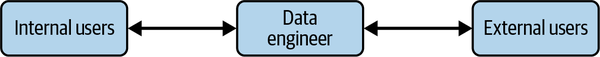
\includegraphics[width=0.92\textwidth, keepaspectratio]{fig_01_09_internal_external_facing.png}
  \caption{A data engineer faces in many directions: external users of products, internal stakeholders, upstream data producers, downstream consumers. Reproduced from Reis \& Housley (2022), Figure~1-9.}
  \label{fig:facing}
\end{figure}

Data engineers don't sit alone. They're at the centre of a web of relationships — with people who produce the data, people who consume it, and people who manage the systems around both. The book splits this into a few sections, and I'll mirror them.

\subsection{Internal-facing vs external-facing data engineers}

A useful distinction the authors make: not all data engineering work is the same.

\begin{itemize}[leftmargin=*]
  \item \textbf{External-facing data engineers} build the data systems behind user-facing products — social networks, IoT platforms, ecommerce. The data they handle includes transactional and event data from those products, and the systems they build often have a feedback loop: data flows from the product into a pipeline and then back into the product (e.g., personalisation features).
  \item \textbf{Internal-facing data engineers} build the data systems that serve internal stakeholders — finance dashboards, ops reporting, internal ML, analyst self-service. Their workloads are typically less concurrent and less latency-sensitive but often more complex in terms of business logic.
\end{itemize}

\begin{figure}[H]
  \centering
  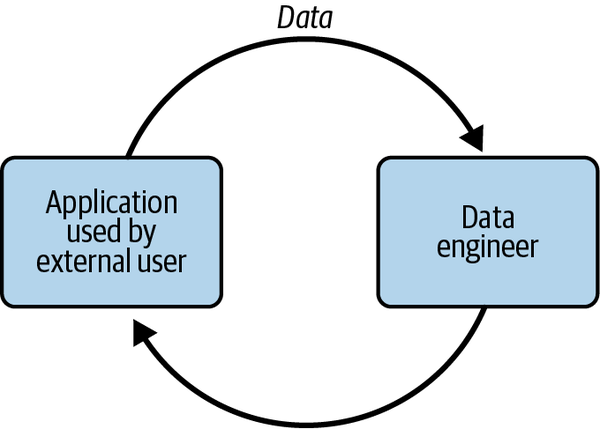
\includegraphics[width=0.65\textwidth, keepaspectratio]{fig_01_10_external_facing_loop.png}
  \caption{The feedback loop in external-facing data systems: data from the product flows through the pipeline and back into the product. Reproduced from Reis \& Housley (2022), Figure~1-10.}
  \label{fig:loop}
\end{figure}

External-facing systems come with a different problem set. Concurrency is much higher (a query engine for an analyst handles dozens of queries; a query engine behind a public-facing app might handle millions). You need tight per-query limits to prevent any single bad actor from blowing up your infrastructure. Multi-tenancy makes security a much harder problem — when one table holds data for thousands of customers, you cannot afford a single ACL miss.

\begin{figure}[H]
  \centering
  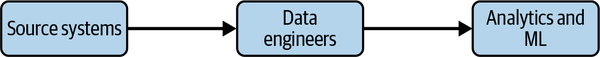
\includegraphics[width=0.92\textwidth, keepaspectratio]{fig_01_11_internal_facing_engineer.png}
  \caption{Internal-facing data engineers serve BI dashboards, ops reports, business processes, data science teams, and ML pipelines. Reproduced from Reis \& Housley (2022), Figure~1-11.}
  \label{fig:internal}
\end{figure}

In practice the two roles bleed together. Internal-facing data is often a prerequisite for external-facing data — your analytics warehouse may also be the source of the features your ML serving layer uses. The relevant question is rarely "internal or external?" but "what are the requirements for this specific dataset?"

\subsection{Data engineers and other technical roles}

\begin{figure}[H]
  \centering
  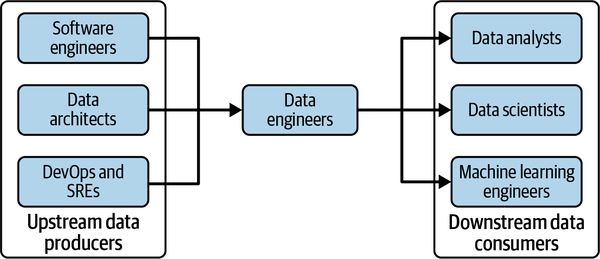
\includegraphics[width=0.92\textwidth, keepaspectratio]{fig_01_12_technical_roles_around_de.png}
  \caption{The technical roles surrounding data engineering. Data engineers sit at the hub between producers and consumers of data. Reproduced from Reis \& Housley (2022), Figure~1-12.}
  \label{fig:roles}
\end{figure}

The book uses the figure above to frame data engineering as a hub: producers (software engineers, data architects, DevOps/SRE) on one side, consumers (analysts, data scientists, ML engineers) on the other. Operational interlocutors (DevOps engineers, again) sit alongside.

\subsubsection{Upstream stakeholders}

These are the people producing the data that the data engineering team consumes. The three the book calls out:

\textbf{Data architects.} An architect operates one level of abstraction up from a data engineer. They design the blueprint — how data flows across silos, what the overall enterprise data architecture looks like, how strategy plays into structure. Good architects come from heavy engineering backgrounds; their value is in being able to translate engineering reality up to leadership and translate strategic goals down into technical decisions.

The cloud has shifted the boundary between architecture and engineering. In the on-prem era, an architect would spend months on a major decision — vendors, contracts, hardware install, capacity planning — and the engineer would implement against that decision. In the cloud era, you can stand up a Snowflake account in an afternoon and start migrating data the next day. Architecture decisions are now often made during implementation, not before it. The roles still exist, but the boundary is more fluid.

\textbf{Software engineers.} They build the application systems that generate most internal data. Application event logs, transactional databases, internal API responses — these are the raw data sources for the analytics and ML systems data engineers build downstream. The book's recommendation is that data engineers and software engineers should coordinate \emph{from the start} of a new project: the worst data pipelines are the ones bolted onto applications that weren't designed with downstream consumption in mind.

A practice that's caught on in the past few years and the book doesn't quite name: \term{data contracts}. The idea is that the schema of an event or table is treated as an explicit, versioned, breakage-trackable interface between the producing software engineer and the consuming data engineer. Chad Sanderson (one of the practitioners the authors thank) has written extensively on this — \href{https://dataproducts.substack.com/}{his Substack} is a good entry point.

\textbf{DevOps engineers and SREs.} They produce data through operational monitoring (logs, metrics, traces) and they often consume it through dashboards. They're upstream and downstream simultaneously. Coordination here matters because operational data systems share a lot of patterns with analytics data systems but are typically run by different teams with different tooling.

\subsubsection{Downstream stakeholders}

These are the people consuming the data the engineers produce.

\textbf{Data scientists.} Build forward-looking models — predictions, recommendations, classifications. Their models scoring live data drive a wide range of products: personalisation, fraud detection, dynamic pricing, recommendations. The book's view, which I share, is that data scientists \emph{shouldn't} spend the bulk of their time on data prep. Engineers should automate enough of the prep work that scientists can spend their time on the modelling itself.

\textbf{Data analysts (or business analysts).} Past- and present-focused, where data scientists are future-focused. They run SQL against the warehouse, build dashboards in BI tools (Tableau, Power BI, Looker, Hex, Mode, Metabase), and turn ambiguous business questions into answers. Their domain expertise is a massive asset — they tend to know the data better than anyone, including the engineers, because they're in it every day. Smart data engineers treat senior analysts as collaborators on data quality.

\textbf{Machine learning engineers (and AI researchers).} ML engineering overlaps with both data engineering and data science. The role takes models from research-y prototypes to production systems — training pipelines, feature stores, model serving, monitoring. The skill set leans heavily on \term{MLOps} practices: CI/CD for models, model versioning, drift detection, A/B testing infrastructure.

The boundary between data engineering, ML engineering, and data science is genuinely blurry, and which work falls to which team depends on the company's structure. At smaller companies one engineer may do all three; at larger ones the roles separate.

AI researchers — at OpenAI, Anthropic, DeepMind, Google Research, FAIR, academia — work on advancing the underlying ML techniques themselves. The book's mention of GPT-3, GPT-4, DALL-E, AlphaGo, and Gato AI as examples is dated now (we're four years on; the frontier has moved several times), but the structural point still holds: research roles are well-resourced and typically operate with engineering support teams.

\subsection{Data engineers and business leadership}

Data engineers increasingly interact with the executive layer — not just because of the business' strategic dependence on data, but because data initiatives have grown big enough to warrant C-level sponsorship.

\subsubsection{The C-suite}

The book runs through the executives a senior data engineer is likely to encounter:

\begin{itemize}[leftmargin=*]
  \item \textbf{CEO} — at non-tech companies, doesn't get into the weeds of data tooling. At tech companies, may be intimately involved. Either way, the data engineering function is the source of "what's possible with the data we have," which feeds vision and strategy.
  \item \textbf{CIO} — owns internal IT. Sets policy, manages the IT budget, supervises ERP, CRM, internal infrastructure. Cloud migrations are often CIO-led. In data-mature orgs, the CIO works closely with data engineering leadership.
  \item \textbf{CTO} — owns external technology strategy: mobile, web, IoT, customer-facing systems. The CTO is responsible for the systems that generate most of the data the data engineers consume, so coordination matters. Data engineering often reports through the CTO at smaller companies.
  \item \textbf{CDO (Chief Data Officer)} — first created at Capital One in 2002. Responsible for data as a corporate asset and for data strategy. Some CDOs supervise data engineering directly; others focus on the strategic and governance side and leave the engineering function to a CTO or CIO.
  \item \textbf{CAO (Chief Analytics Officer)} — focuses on analytics, decision-making, and the analytics function. Where both CDO and CAO exist, the CDO leans toward technology and the CAO leans toward business analysis.
  \item \textbf{CAO-2 (Chief Algorithms Officer)} — newer role, focused on data science and ML. Typically held by someone with deep ML background and an advanced research degree.
\end{itemize}

If the proliferation of "Chief X Officer" titles feels like it's getting out of hand — that's because it is. The book lists six C-suite titles potentially relevant to data work, and which set of them an organisation has tells you something about how seriously, and how chaotically, that organisation takes data.

\subsubsection{Project and product managers}

\textbf{Project managers} run programs — they direct traffic, prioritise the backlog, plan sprints, and report progress to stakeholders. Most run some flavour of Agile/Scrum. Data engineering work often spans multi-quarter initiatives (a cloud migration, a new pipeline architecture, a major schema overhaul), and project managers keep these on track.

\textbf{Product managers} own product lines. In a data-engineering context this often means \term{data products} — datasets, dashboards, ML features, or APIs treated as first-class products with users and SLAs. Data product management is itself an emerging role; \href{https://martinfowler.com/articles/data-mesh-principles.html}{Zhamak Dehghani's data mesh writing} treats the product orientation as a foundational principle.

\textbf{Other management.} The remaining managers a data engineer interacts with — engineering managers, operations managers, finance partners — generally engage through one of two service models: a \textbf{centralised data team} that takes in requests from across the org, or a \textbf{cross-functional embed} where data engineers are assigned to specific business units. Both work. Both have characteristic failure modes (the central team that becomes a bottleneck; the embedded engineer who loses connection to data engineering best practices). Knowing which model your org uses, and adapting to it, matters more than which one is "best."

\section{Conclusion — what to take away}

The chapter is doing a lot of work and it's worth pausing to summarise what I want to remember.

\begin{defbox}
\textbf{Key takeaways from Chapter 1}

\begin{enumerate}[leftmargin=*]
  \item \textbf{Definition.} Data engineering is the development, implementation, and maintenance of systems and processes that turn raw data into high-quality information for downstream consumers.
  \item \textbf{The lifecycle.} Five stages — generation, storage, ingestion, transformation, serving — threaded by six undercurrents — security, data management, DataOps, architecture, orchestration, software engineering.
  \item \textbf{The arc.} Data warehousing (1980s) → web-era scaling (1990s) → big-data-era distributed computing (2000s) → cloud-era simplification and the modern data stack (2010s--2020s).
  \item \textbf{Scientists and engineers.} Data engineering sits upstream of data science. Engineers provide the foundation; without it, scientists become reluctant data engineers.
  \item \textbf{Maturity matters.} Stage 1 (starting) needs generalists who avoid heavy lifting. Stage 2 (scaling) needs formal practices and specialists. Stage 3 (leading) needs custom tools and a culture against complacency.
  \item \textbf{Type A vs Type B.} Type A composes existing pieces. Type B builds new pieces. Most engineers are A; most companies need a few B's where competitive advantage is at stake.
  \item \textbf{The role is connective.} Data engineers sit at the centre of a web — software engineers and architects upstream, analysts/scientists/ML engineers downstream, executives and product managers around all of it. The technical skills are necessary but not sufficient.
\end{enumerate}
\end{defbox}

\section{Additional resources I'm filing for later}

The book ends each chapter with an "Additional Resources" list. Some I've already woven into these notes; here's the consolidated list, with a note for each on why it's worth reading.

\begin{itemize}[leftmargin=*]
  \item \textbf{Maxime Beauchemin, \href{https://www.freecodecamp.org/news/the-rise-of-the-data-engineer-91be18f1e603/}{"The Rise of the Data Engineer"} (2017).} The piece that named the field. Mandatory.
  \item \textbf{Maxime Beauchemin, \href{https://maximebeauchemin.medium.com/the-downfall-of-the-data-engineer-5bfb701e5d6b}{"The Downfall of the Data Engineer"} (2017).} The follow-up. A more pessimistic and arguably more accurate take on the burnout patterns in the role.
  \item \textbf{Monica Rogati, \href{https://hackernoon.com/the-ai-hierarchy-of-needs-18f111fcc007}{"The AI Hierarchy of Needs"} (2017).} The hierarchy that explains why ML projects fail without good data engineering.
  \item \textbf{Robert Chang, \href{https://medium.com/@RobertChang/doing-data-science-at-twitter-49ac2bf0edae}{"Doing Data Science at Twitter"} (2015).} The article where the type A / type B split was introduced.
  \item \textbf{Jordan Tigani, \href{https://motherduck.com/blog/big-data-is-dead/}{"Big Data is Dead"} (2023).} A useful corrective to the lingering big-data orthodoxy.
  \item \textbf{Lewis Gavin, \emph{What Is Data Engineering?} (O'Reilly, 2020).} A short, free book covering the same territory at a higher level. Useful as an alternative angle.
  \item \textbf{Jesse Anderson, \emph{Data Teams} (Apress).} On structuring and growing data teams.
  \item \textbf{John Thompson, \emph{Building Analytics Teams} (Packt).} Companion to Anderson on team building from the leadership side.
  \item \textbf{Martin Kleppmann, \emph{Designing Data-Intensive Applications} (O'Reilly).} Not on the book's list but absolutely required reading. The systems-engineering view of the same field.
  \item \textbf{Zhamak Dehghani, \emph{Data Mesh} (O'Reilly).} On the decentralised, domain-oriented data architecture pattern.
  \item \textbf{Chad Sanderson, \href{https://dataproducts.substack.com/}{Data Products Substack}.} The home of the data contracts conversation.
  \item \textbf{The DataOps Manifesto.} \url{https://dataopsmanifesto.org/} — the reference document for the DataOps undercurrent.
\end{itemize}

\section{Videos, talks, and podcasts I'm queuing up}

The book leans on written sources for its references. I want to add a video/podcast layer on top, because some of these ideas land harder when you hear the practitioners talking through them. I've grouped these by topic so I can pull the right one when I'm reviewing a section.

\subsection*{On the field, the role, and how it got here}

\begin{itemize}[leftmargin=*]
  \item \textbf{The Joe Reis Show} --- \href{https://www.youtube.com/@JoeReisData}{youtube.com/@JoeReisData}. The author's own show. Episodes with Bill Inmon, Zhamak Dehghani, Maxime Beauchemin, and Jordan Tigani are the highest-leverage starting points.
  \item \textbf{Maxime Beauchemin, ``The Rise of the Data Engineer''} --- talks at Strata, Coalesce, and Data Council. The conference-recording versions extend the article and add Q\&A.
  \item \textbf{Maxime Beauchemin, ``The Downfall of the Data Engineer''} --- the follow-up talk on the burnout patterns in the role.
  \item \textbf{Bill Inmon \& Joe Reis on the data lakehouse} --- Inmon, who coined ``data warehouse'' in 1989, has a co-authored book with Reis on the lakehouse. The corresponding podcast episodes are an unusual chance to hear a forty-year practitioner's view of where storage architecture is heading.
\end{itemize}

\subsection*{On the historical arc — warehousing, big data, the cloud}

\begin{itemize}[leftmargin=*]
  \item \textbf{Andy Pavlo's CMU Intro to Database Systems (15-445)} --- \href{https://www.youtube.com/@CMUDatabaseGroup}{youtube.com/@CMUDatabaseGroup}. Lectures on relational model, storage, indexing, query processing, transactions. Free. There's also \textbf{15-721 Advanced Database Systems}, which goes deep into OLAP, vectorisation, query optimisation, and the modern columnar/lakehouse stack — the perfect companion for the technology end of this book.
  \item \textbf{Doug Cutting on the origins of Hadoop} --- several talks online about how the Yahoo! team built Hadoop from the Google papers. \href{https://www.youtube.com/results?search_query=doug+cutting+hadoop}{YouTube has multiple recordings.}
  \item \textbf{Werner Vogels on building AWS} --- the AWS CTO's talks at re:Invent each year are a long history of cloud-data infrastructure. The early talks (2011--2014) document the origin story of S3, EC2, and DynamoDB.
  \item \textbf{Jordan Tigani, ``Big Data is Dead''} --- the talk version of the MotherDuck blog post. Several conference recordings.
\end{itemize}

\subsection*{On data mesh, data products, and modern architecture}

\begin{itemize}[leftmargin=*]
  \item \textbf{Zhamak Dehghani on data mesh} --- \href{https://www.youtube.com/watch?v=TVxdW2gG3X8}{her InfoQ talk}, plus the longer keynote series at Data Council and Subsurface.
  \item \textbf{Chad Sanderson on data contracts} --- talks at dbt Coalesce and Data Council on treating dataset schemas as explicit, versioned producer/consumer contracts.
  \item \textbf{Benn Stancil's writing and talks} --- Benn is one of the more thoughtful voices in modern data; his \href{https://benn.substack.com/}{Substack} is essential. Several of his talks from Coalesce are on YouTube.
  \item \textbf{Tristan Handy / dbt Labs talks} --- worth tracking for the modern data stack perspective. Tristan's annual ``state of analytics engineering'' talks are a good barometer of where the dbt-flavoured side of the field is going.
\end{itemize}

\subsection*{On the systems-engineering foundations}

\begin{itemize}[leftmargin=*]
  \item \textbf{Martin Kleppmann, ``Turning the database inside out''} (Strange Loop 2014) --- \href{https://www.youtube.com/watch?v=fU9hR3kiOK0}{youtube.com}. The talk that informally introduced log-based, stream-first thinking to a wide audience. Pair with his book.
  \item \textbf{Jay Kreps's ``The Log: What every software engineer should know''} --- the LinkedIn-era essay that became a foundational reading for the streaming side of data engineering. \href{https://engineering.linkedin.com/distributed-systems/log-what-every-software-engineer-should-know-about-real-time-datas-unifying}{linkedin.com/engineering}.
  \item \textbf{Jepsen / Kyle Kingsbury's database analyses} --- when consistency, isolation, and distributed correctness matter, Jepsen is the reference. \href{https://jepsen.io/analyses}{jepsen.io/analyses}.
\end{itemize}

\subsection*{On data quality, observability, and governance}

\begin{itemize}[leftmargin=*]
  \item \textbf{Barr Moses (Monte Carlo) on data observability} --- talks at Coalesce, Data Council, and Subsurface explaining the observability framework and the ``five pillars'' of data quality.
  \item \textbf{Andrew Ng, ``MLOps: From Model-Centric to Data-Centric AI''} --- the talk that flipped the field's attention from model tuning to data quality. \href{https://www.youtube.com/watch?v=06-AZXmwHjo}{youtube.com}.
\end{itemize}

\subsection*{On business / executive dynamics around data}

\begin{itemize}[leftmargin=*]
  \item \textbf{Tom Davenport's talks on data leadership} --- particularly his work on ``data-driven culture'' and the role of executives in driving data initiatives. He co-authored the HBR piece the book references.
  \item \textbf{Cassie Kozyrkov on decision intelligence} --- a clean framing of the gap between analytics output and business decisions. Her YouTube series \emph{Making Friends with Machine Learning} is excellent.
\end{itemize}

\section{A short glossary I made for myself}

Some of the terms that come up repeatedly in this chapter and the next, with my one-line summaries. I'll extend this as I move through the book.

\begin{description}[leftmargin=2cm, style=nextline]
  \item[Data engineering] Building and operating systems that turn raw data into reliable, governed information for downstream consumers.
  \item[Data engineering lifecycle] The five stages (generation $\to$ storage $\to$ ingestion $\to$ transformation $\to$ serving) and six undercurrents (security, data management, DataOps, architecture, orchestration, software engineering) that the book uses as its organising frame.
  \item[Source system] A system that produces data — application database, event stream, IoT device, third-party API, file feed.
  \item[OLTP] Online Transaction Processing. Operational databases optimised for high-concurrency, small-transaction workloads (e.g. Postgres, MySQL backing a web app).
  \item[OLAP] Online Analytical Processing. Workloads optimised for large scans, aggregations, and analytical queries (e.g. Snowflake, BigQuery, ClickHouse).
  \item[ETL / ELT] Extract-Transform-Load vs Extract-Load-Transform. ETL was the on-prem default; ELT is the cloud-warehouse default. dbt is the canonical ELT-style transformation tool.
  \item[Data warehouse] A central, schema-defined, query-optimised analytical store. Inmon and Kimball gave us the two dominant modelling philosophies.
  \item[Data lake] Raw or semi-structured data stored in object storage (S3, GCS, ADLS). Cheap, flexible, but historically harder to query consistently.
  \item[Lakehouse] A pattern that brings ACID transactions, schema evolution, and time travel to data-lake storage via open table formats (Delta Lake, Apache Iceberg, Apache Hudi). Often pitched as ``warehouse semantics on lake economics.''
  \item[Modern data stack] The current default toolkit for analytics-focused data work: cloud warehouse + ELT ingestion (Fivetran/Airbyte) + dbt for transformation + BI tool + orchestrator (Airflow/Dagster/Prefect).
  \item[Data mesh] An architectural pattern that decentralises data ownership to domain teams and treats datasets as products with explicit contracts. Coined by Zhamak Dehghani.
  \item[Data observability] Monitoring data quality and freshness the way DevOps monitors application health. Five pillars: freshness, distribution, volume, schema, lineage.
  \item[Data contract] An explicit, versioned schema agreement between a data producer and consumers, with breakage SLAs.
  \item[DataOps] Applying DevOps practices (CI/CD, observability, version control, automated testing) to data systems. \href{https://dataopsmanifesto.org/}{The DataOps Manifesto} is the reference.
  \item[Reverse ETL] Pushing transformed/curated data back \emph{out} of the warehouse into operational systems (Salesforce, Marketo, ad platforms). Tools: Hightouch, Census.
  \item[Type A / Type B data engineer] Type A composes existing tools; Type B builds new ones.
\end{description}

\bigskip
\hrule
\bigskip

\noindent\emph{Next up: Chapter 2 — the data engineering lifecycle in proper depth. The skeleton I sketched in this chapter gets its full anatomy.}

\clearpage


\end{document}
